\documentclass[a4paper,10pt]{article}

\usepackage{ucs}
\usepackage[utf8x]{inputenc}
\usepackage[english]{babel}
\usepackage{fontenc}
\usepackage{graphicx}
\usepackage[a4paper, top=2cm]{geometry}

\usepackage[dvips]{hyperref}
\title{String Algorithms 2013 - Assignment 2}
\author{Holger Schmeisky  201211113, Tashi Sherpa, Matus Tomlein 201210962}
\date{30.04.2013}

\begin{document}

\maketitle

\subsection*{State of the algorithm}
The algorithm works correctly for all inputs specified on the homepage, and thus we think it works correctly on all inputs.

\subsection*{Insights}
While implementing the algorithm we got a deeper understanding of its working.\\ 
It was very helpful to draw an execution of the algorithm on paper. After we did this, we saw how with the mapping of DFS-traversal numbers to leaf indices, we could very simply calculate the leaf lists of inner nodes as intervals between the DFS-traversal numbers. Before we thought it would be difficult to calculate and store, $LL(n)$ and $LL'(n)$, but with the paper drawing, we saw that after we had traversed all of an inner node's children, we had all the information we needed, to determine the largest subtree (the one with the largest interval) and to store that as interval. In the later iteration through the inner node's leaflist, we could just skip the indices in the $LL(n)$ interval.

\subsection*{Problems}
We did not really face any big problems, after the preliminary observations made on paper. We developed the algorithm by first testing it on small input examples (``abaab'') until it produced the correct leaf lists and repeats there and subsequently fed it with larger inputs. Each of the larger inputs discovered new programming errors, but we were able to get it working relatively quickly on all of the inputs on the homepage.

\clearpage
\subsection*{Evaluation}
We evaluated our implementation using a script that gradually increased the
length of the input.
It increased the input string size by 5000 characters each time until it
reached the length of 147481 characters.
The input was a sample DNA string.
For each input size we measured the running time 10 times and calculated
an average running time.

The results can be seen on figure~\ref{fig:evaluation}.
Although we calculated the running time as an average of 10 measurements,
the results sometimes decrease for bigger inputs as can be seen on the graph.

The graph shows that the running time does not increase in $O(n^2)$ fashion.
The $O(n*log(n))$ running time would probably be more evident for larger
inputs.

\begin{figure}
\centering
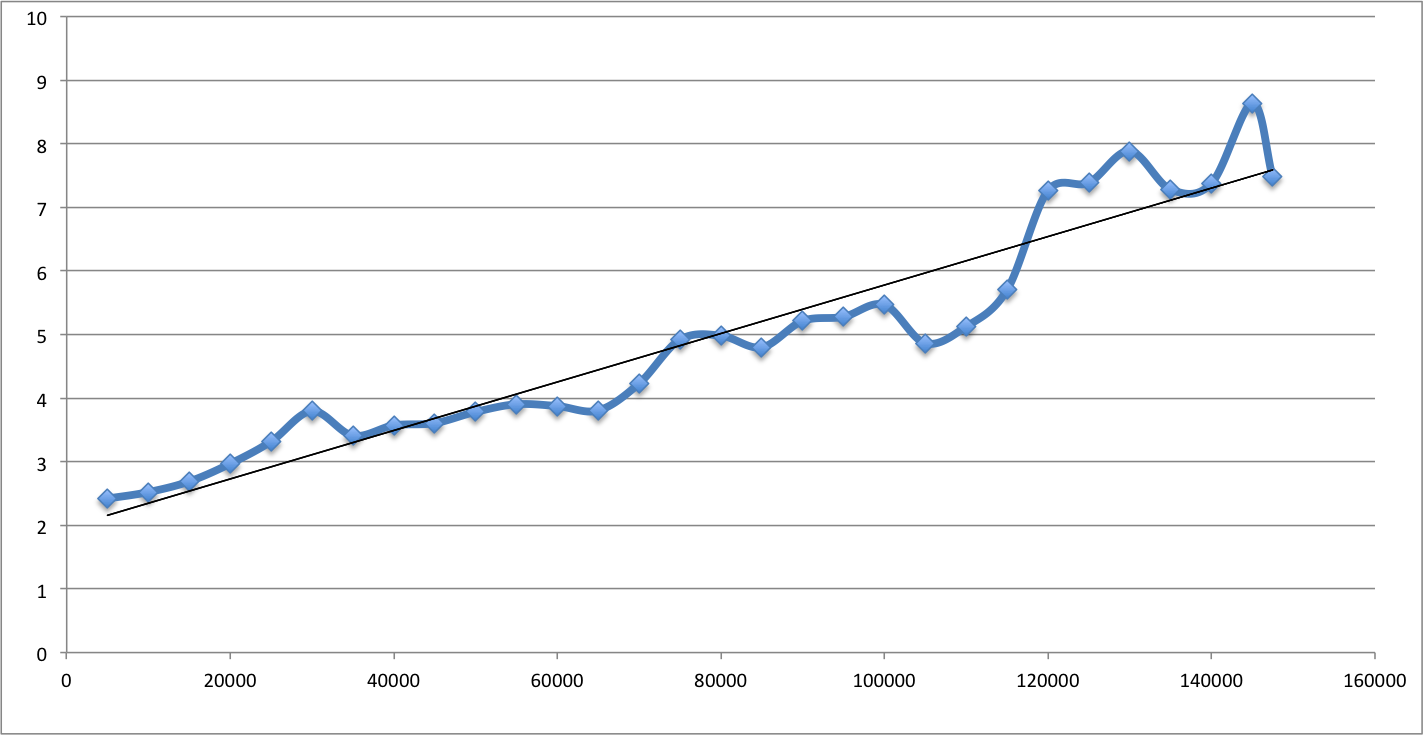
\includegraphics[scale=0.6]{images/tandem-evaluation_graph.png}
\caption{Plot of measured running times. The Y-axis shows the running times
in seconds and the x-axis shows the length of the input in characters.}
\label{fig:evaluation}
\end{figure}

\end{document}
